\documentclass[conference]{IEEEtran}

\usepackage{cite}
\usepackage{amsmath,amssymb,amsfonts}
\usepackage{algorithmic}
\usepackage{graphicx}
\usepackage{textcomp}
\usepackage{xcolor}
\documentclass[12pt,a4paper]{article}
\usepackage{graphicx} % Required for including images
\usepackage{xcolor}   % For custom colors in code boxes
\usepackage[utf8]{inputenc}
\usepackage{listingsutf8} % For code formatting with UTF-8 support
\usepackage{graphicx}
\usepackage{tikz}
\usepackage{hyperref}
\usepackage{listings}
\usepackage[most]{tcolorbox}
\usepackage{tcolorbox} % For boxed content
\usepackage[utf8]{inputenc}
\usepackage{geometry} % To set page margins
\usepackage{setspace} % For line spacing
\usepackage{setspace} % For line spacing
\geometry{a4paper, margin=1in}

\usepackage{tcolorbox} % For boxed content
\usepackage[utf8]{inputenc}
\usepackage{geometry} % To set page margins
\usepackage{setspace} % For line spacing
\usepackage{setspace} % For line spacing
\geometry{a4paper, margin=1in}

\lstset{
    language=Python,
    basicstyle=\ttfamily\footnotesize,
    keywordstyle=\color{blue}\bfseries,
    commentstyle=\color{green!50!black},
    stringstyle=\color{red},
    frame=single,
    breaklines=true,
    showstringspaces=false,
    numbers=left,
    numberstyle=\tiny,
    stepnumber=1,
    numbersep=5pt
}

\def\IEEEtitletopspace{10mm}

\begin{document}

\title{Quantum Cloud Integration: Potential Impact of Quantum Computing on Cloud Storage}

\author{
    \IEEEauthorblockN{Priyanshu Kumar Sharma, Neha Gaikwad, Krishna Pandey, Paavani Bargoti}
    
    \vspace{10pt} % Adds some space between authors and the guide
    \IEEEauthorblockN{Guide: Prini Rastogi}
    \IEEEauthorblockA{
        \textit{Ajeenkya D Y Patil University} \\
        Pune, India \\
        Email: prini.rastogi@inurture.co.in
    }
}

\maketitle

\begin{abstract}
The \textbf{Quantum Cloud Integration: Potential Impact of Quantum Computing on Cloud Storage} project investigates the synergistic integration of quantum computing capabilities with classical cloud infrastructure, aiming revolutioniseize storage and data processing paradigms. Quantum computing, known for its ability to tackle complex computational problems, is poised to complement the scalability and accessibility of classical cloud systems. This project highlights a hybrid architecture designed to enhance cloud storage efficiency, data security, and processing capabilities, leveraging quantum algorithms alongside traditional computational methods.  

Key components of the project include:  \\
1. \textbf{Quantum Workflow Implementation}: Quantum circuits are developed using Python and Qiskit to address specific computational tasks, such as optimizing data compression, encryption, and retrieval. The circuits interact seamlessly with classical resources, ensuring a hybrid computational workflow.  \\
2. \textbf{Dockerized Integration Framework}: The entire system is containerized using Docker, enabling modularity, portability, and simplified deployment of hybrid quantum-cloud applications. This framework bridges the gap between classical cloud resources and quantum backends.  \\
3. \textbf{Hybrid Resource Management}: The integration employs AWS for managing classical tasks, such as scalable storage and data handling, while IBM Quantum processes quantum-specific computations, such as Shor’s algorithm for factorization and Grover’s algorithm for search optimization.  \\
4. \textbf{Secure Communication Protocols}: Advanced encryption and secure socket communication ensure robust data transfer between the classical and quantum systems, mitigating potential vulnerabilities in hybrid workflows.  

The system demonstrates groundbreaking use cases, such as efficient data encryption using quantum key distribution (QKD), quantum-enhanced data indexing for cloud storage, and optimized workload distribution across hybrid resources. Challenges addressed include mitigating noise in amount  calculations, managing classical- to- amount transitions, and  icing real- time responsiveness in cold-blooded  tasks. 
 
 This  exploration underscores the transformative  eventuality of amount computing in reshaping  pall  storehouse strategies. It highlights how cold-blooded  systems can achieve  unequaled   effectiveness and security, paving the way for innovative  pall  infrastructures able of handling  unborn data demands in a amount  period. 

\end{abstract}

\begin{IEEEkeywords}
Quantum computing, Cloud integration, Hybrid architecture, Quantum algorithms, Cloud systems.
\end{IEEEkeywords}

\section{Introduction}
 Quantum computing is poised to revolutionize various fields by solving complex problems at speeds far exceeding traditional computing. Unlike classical systems, which use binary bits, quantum computing relies on quantum bits (qubits) that can exist in multiple states simultaneously, offering exponential advantages for tasks like encryption, optimization, and data analysis. Cloud computing, on the other hand, provides scalable, accessible, and cost-efficient resources for data storage and processing. However, traditional cloud systems are reaching their limits in handling complex tasks, especially those requiring high computational power or advanced security.

    Quantum-cloud integration combines the strengths of both quantum and classical systems to address these limitations. By leveraging quantum computing for high-complexity operations such as encryption, data searching, and optimization, and using classical systems for routine tasks, this hybrid approach can enhance cloud storage and computing. Quantum algorithms, like Grover’s for faster searches and Shor’s for breaking encryption, promise to significantly improve cloud system capabilities.
    
    This research explores the implementation of quantum-cloud integration using tools like IBM Quantum for quantum algorithms, AWS for classical computing, and Docker for containerization. The goal is to create a modular, secure, and efficient system that can handle complex workloads. While challenges such as qubit coherence and system integration remain, the potential impact of this integration on industries such as healthcare, finance, and scientific research is profound. By examining both the openings and hurdles, this design aims to contribute to the development of unborn pall systems powered by amount computing.
    
\subsection{Core Concepts of Quantum-Cloud Integration}
Quantum-cloud integration is a multidisciplinary field that combines principles from quantum computing, cloud computing, and cybersecurity. Key concepts include:

\begin{itemize}
    \item \textbf{Quantum Computing}: Utilizes qubits to achieve parallelism through superposition and entanglement, enabling exponential computational speedups for specific tasks.
    \item \textbf{Cloud Computing}: Offers scalable, flexible, and cost-effective solutions for data storage and processing, essential for businesses and individual users.
    \item \textbf{Hybrid Model}: Combines quantum and classical resources, leveraging the strengths of both paradigms to optimize performance and efficiency.
\end{itemize}

\section{Quantum Computing}

Quantum computing represents a paradigm shift in computational power, using the principles of amount mechanics. In this section, we will explore the abecedarian generalities of amount computing, its comparison with traditional computing, and the tools available for amount programming, similar as Qiskit

\subsection{Why Quantum Computing?}
Quantum computing is not just an incremental improvement over classical computing; it promises to solve problems that are currently intractable. Problems in areas like cryptography, optimization, and simulations can benefit from quantum algorithms that leverage superposition and entanglement, two key principles of quantum mechanics. These properties allow quantum computers to explore multiple solutions simultaneously, drastically reducing the time required for problem-solving in some cases.

\subsection{Quantum Computing v/s Traditional Computers}
 Classical computers use  double bits( 0 or 1) for  calculation, whereas amount computers use amount bits, or qubits, which can  live in multiple  countries at  formerly due to superposition. This leads to exponential speedups for certain classes of problems. 


\subsection{Traditional Computers: Mathematical Operations}

In traditional computers, calculations are based on \textbf{classical bits}, which represent either 0 or 1. These bits undergo basic operations such as AND, OR, NOT, and XOR, forming the foundation for complex computations.

\subsubsection{Key Operations:}

\begin{itemize}
    \item \textbf{Addition (Binary Addition):}
    \begin{itemize}
        \item The binary addition of two bits follows basic rules:
        \begin{enumerate}[noitemsep]
    \item Adding rightmost bits: \(1 + 1 = 10\), write \(0\), carry \(1\).
    \item Next bits: \(0 + 1 + 1 (\text{carry}) = 10\), write \(0\), carry \(1\).
    \\
    \item Repeat until leftmost bits, adding the final carry.
\end{enumerate}
    \end{itemize}
    
    \item \textbf{Multiplication (Binary Multiplication):}
    \begin{itemize}
        \item Binary multiplication is similar to decimal multiplication but uses the rules for binary digits.
        \item Example:
        \[
        1101 \ (\text{13 in decimal}) \\
        \times 1011 \ (\text{11 in decimal}) \\
        
        \\
        % &\text{Final result:} \quad 10011111 \quad (\text{143 in decimal})
        \]
    \end{itemize}
    
    \item \textbf{Bitwise Operations:}
    \begin{itemize}
        \item \textbf{AND:} 
        \[
        1 \ \text{AND} \ 1 = 1, \quad \text{else} \ 0
        \]
        \item \textbf{OR:} 
        \[
        1 \ \text{OR} \ 0 = 1, \quad \text{else} \ 0
        \]
        \item \textbf{NOT:} Inverts the bit: 
        \[
        \text{NOT} \ 0 = 1, \quad \text{NOT} \ 1 = 0
        \]
        \item \textbf{XOR:} 
        \[
        1 \ \text{XOR} \ 1 = 0, \quad 0 \ \text{XOR} \ 0 = 0, \quad 1 \ \text{XOR} \ 0 = 1 
        \]
    \end{itemize}

    \item \textbf{Shift Operations:}
    \begin{itemize}
        \item \textbf{Left Shift ($\ll$):} Moves all bits to the left, adding zeros to the right.
        \[
        1010 \ll 1 = 10100
        \]
        \item \textbf{Right Shift ($\gg$):} Moves all bits to the right, discarding the rightmost bits.
        \[
        1010 \gg 1 = 0101
        \]
    \end{itemize}
\end{itemize}

These operations are abecedarian to all computational tasks in traditional computers, similar as computation, sense, data storehouse, and reclamation. still, they come hamstrung for large- scale or complex problems that bear exponential computational growth.

\subsection{Qiskit: Quantum Programming Framework}

\begin{tcolorbox}[title=Qiskit Example]
\begin{lstlisting}[language=Python]
from qiskit import QuantumCircuit, Aer, execute

# Create a simple quantum circuit with two qubits
qc = QuantumCircuit(2, 2)
qc.h(0)  # Apply Hadamard gate
qc.cx(0, 1)  # Apply CNOT gate
qc.measure([0, 1], [0, 1])

# Simulate the circuit
simulator = Aer.get_backend('qasm_simulator')
result = execute(qc, simulator, shots=1024).result()

# Display results
counts = result.get_counts()
print("Quantum Results:", counts)
\end{lstlisting}
\end{tcolorbox}
Qiskit is an open- source amount computing software development  frame developed by IBM. It allows  druggies to write amount algorithms,  pretend amount circuits, and run them on real amount computers. The reasons to use Qiskit include its comprehensive set of tools, ease of integration with other platforms, and access to IBM's amount  tackle for real- world  operations. The above code is the simple  illustration of an amount circuit created using Qiskit

Qiskit allows druggies to design and pretend amount algorithms without taking advanced knowledge of amount drugs.

\subsection{Qubits v/s Traditional Bits}
 Traditional computers use bits to represent information, where each bit can either be 0 or 1. On the other hand, qubits( amount bits) are the  introductory unit of amount computing, which can  live in a superposition of both 0 and 1  countries  contemporaneously. This property, along with amount trap, allows amount computers to  break certain types of problems exponentially  briskly than classical computers. 


Here is a graphical representation comparing bits and qubits:

\begin{figure}[h!]
    \centering
    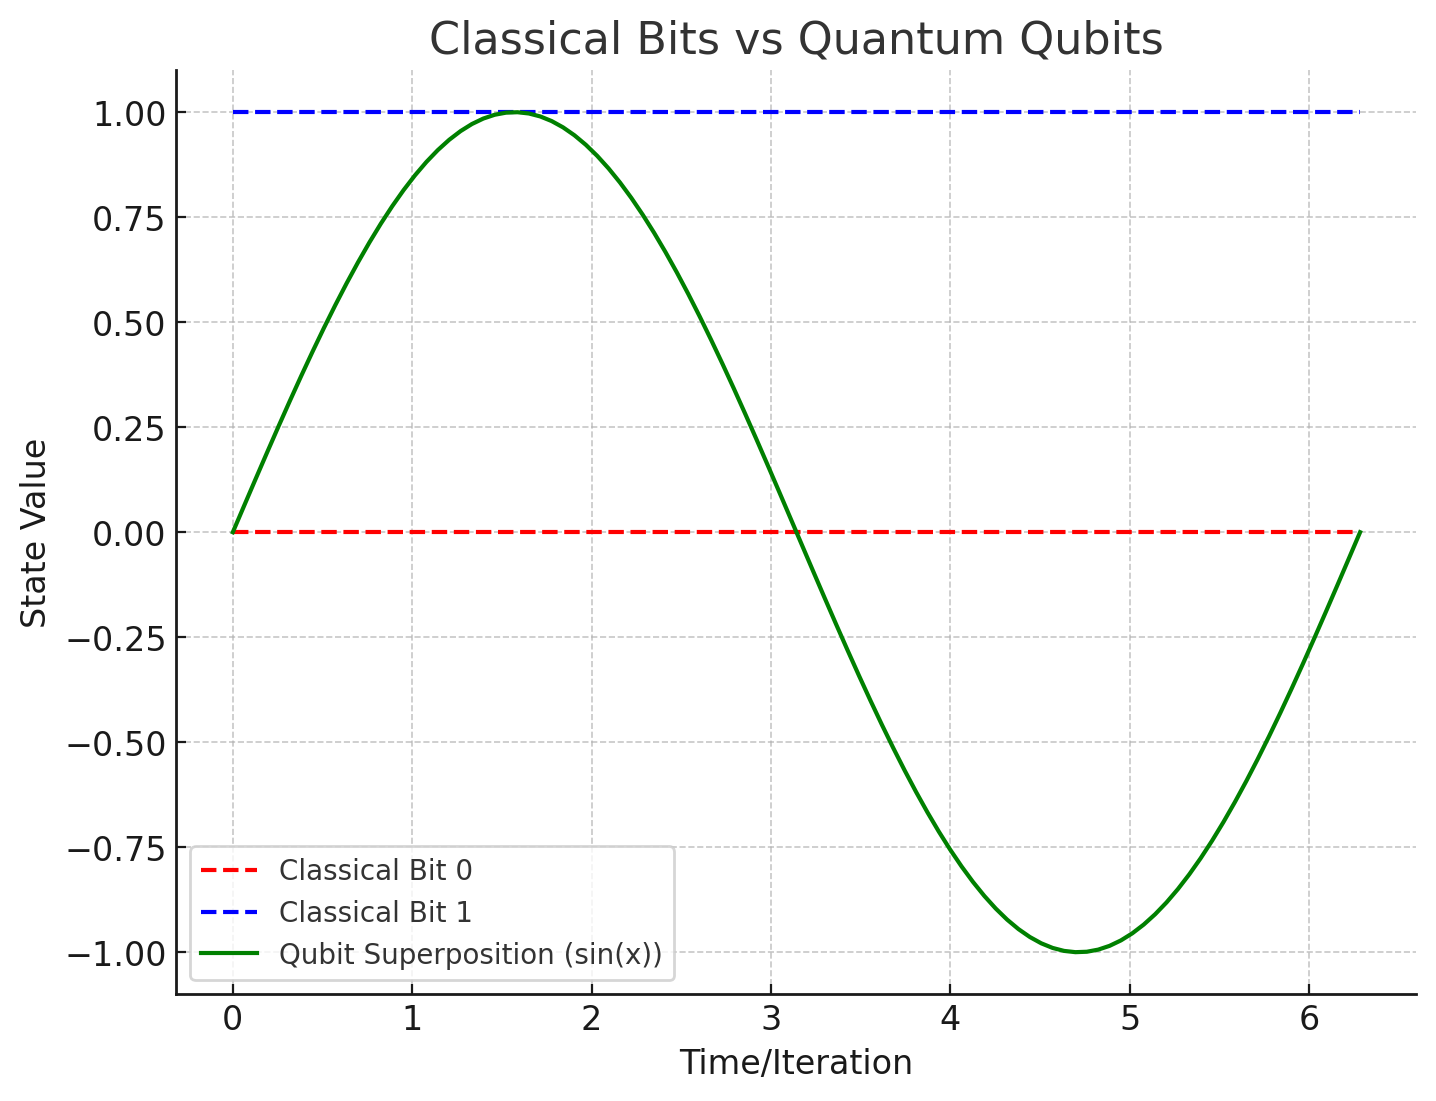
\includegraphics[width=0.5\textwidth]{D:/SEM-5/FSDC/quantum-cloud-integration/images/qubits_vs_bits.png}
    \caption{Comparison of Qubits and Bits}
    \label{fig:qubits_vs_bits}
\end{figure}


\begin{center}
    \fontsize{14}{16}\selectfont \bfseries
    \section{Quantum Computing Applications}
\end{center}
Quantum computing has the implicit to revise  colorful fields by  working complex problems that are  presently  unattainable 
 with classical computers. Some of the  crucial  operations of amount computing include 

\begin{itemize}
\item \textbf{Cryptography:} Quantum computers can potentially break many encryption algorithms currently in
use, but they can also be used to create unbreakable encryption methods.
\item \textbf{Optimization:} Quantum computers can quickly find the optimal solution to complex
optimization problems, which can be used in fields such as logistics, finance, and energy management.
\item \textbf{Simulation:} Quantum computers can simulate complex quantum systems, which can be used in
fields such as chemistry and materials science
\item \textbf{Machine Learning:}Quantum computers can be used to speed up certain machine
literacy algorithms, which can be used in fields similar as image recognition and natural language processing
\end{itemize}


\subsection{Objectives}
This paper aims to:
\begin{itemize}
   \item  Develop a modular armature to integrate amount and classical  pall systems. 
   \item Explore the operation of amount algorithms for tasks like encryption, data hunt, and optimization in pall storehouse.
   \item  Demonstrate the practical feasibility of  mongrel amount-  pall systems using real- world tools. 
   \item  Address Specialized challenges similar as error rates, resource allocation, and communication protocols. 

\end{itemize}

\subsection{Key Features of the Integration Framework}
The project utilizes the following tools and technologies:
\begin{itemize}
    \item \textbf{Secure Communication}:Utilizes encryption ways for secure data transfer between amount and classical systems.
    \item \textbf{Modular Design}: Ensures flexibility and adaptability for various applications.
    \item \textbf{Workflow Optimization}:Allocates tasks to amount or classical systems grounded on computational conditions.
    \item \textbf{Fault Tolerance}: Implements mechanisms to handle quantum system errors and instability.
    
\end{itemize}


\begin{itemize}
    \item \textbf{Quantum Computing: An Overview}
    \begin{itemize}
        \item Quantum computing is grounded on the principles of amount mechanics, similar as superposition, trap, and amount hindrance.
        \item Unlike classical computing, which uses double bits( 0 and 1), amount computing uses qubits that can live in multiple countries contemporaneously.
        \item This allows amount computers to perform certain types of calculations exponentially briskly than classical computers.
    \end{itemize}

    \item \textbf{Qubits vs Traditional Bits}
    \begin{itemize}
        \item \textbf{Traditional Bits:} 
        \begin{itemize}
            \item Represent information as double countries( 0 or 1).
            \item Operate on deterministic systems governed by classical drugs.
            \item Suitable for general- purpose operations but face limitations in handling complex problems like cryptography or large- scale optimizations.
        \end{itemize}
        \item \textbf{Qubits:} 
        \begin{itemize}
           \item Represent Amount countries, allowing superposition( contemporaneous actuality in 0 and 1).
           \item Exploit trap for correlations between qubits, enabling distributed calculations.
           \item Enable community in recycling multiple possibilities at formerly, drastically reducing calculation time for specific problems.
        \end{itemize}
        \item \textbf{Key Comparison:}
        \begin{itemize}
            \item Classical bits are direct and successional; qubits enable exponential scaling in certain calculations.
            \item Quantum systems introduce probabilistic issues, taking technical algorithms to interpret results.
        \end{itemize}
    \end{itemize}

    \item \textbf{Qiskit: Quantum Software Framework}
    \begin{itemize}
        \item Qiskit is an open- source toolkit handed by IBM for developing amount computing operations.
        \item \textbf{Key Features:}
        \begin{itemize}
            \item Tools for erecting amount circuits, running simulations, and executing circuits on IBM Quantum bias.
            \item Access to amount algorithms, similar as Grover's for searching and Shor's for factorization.
        \end{itemize}
        \item \textbf{Example of a Quantum Circuit in Qiskit:}
        \begin{enumerate}
            \item Import necessary libraries: \texttt{from qiskit import QuantumCircuit, Aer, execute}.
            \item Create a quantum circuit: \texttt{qc = QuantumCircuit(2, 2)}.
            \item Add gates:
            \begin{itemize}
                \item Hadamard gate: \texttt{qc.h(0)}.
                \item CNOT gate: \texttt{qc.cx(0, 1)}.
            \end{itemize}
            \item Measure the qubits: \texttt{qc.measure([0, 1], [0, 1])}.
            \item Simulate using Aer and get results: \texttt{execute(qc, simulator).result()}.
        \end{enumerate}
    \end{itemize}

    \item \textbf{Quantum-Cloud Integration}
    \begin{itemize}
        \item A cold-blooded approach combining amount computing's computational power with the scalability of pall computing.
        \item Quantum calculating handles specific high- complexity tasks, similar as encryption, optimization, and simulation.
        \item Cloud computing provides the structure for managing classical tasks like storehouse and resource allocation.
        \item Benefits include:
        \begin{itemize}
            \item Faster data processing for specific workloads.
             \item Enhanced security through amount encryption.
              \item Bettered optimization in resource- ferocious diligence.
        \end{itemize}
    \end{itemize}

    \item \textbf{Challenges in Quantum-Cloud Integration}
    \begin{itemize}
        \item \textbf{Hardware Limitations:}
        \begin{itemize}
            \item Qubit consonance time is short, leading to crimes in long calculations.
            \item Limited vacuity of amount tackle with sufficient qubits.
        \end{itemize}
        \item \textbf{Software and Algorithmic Barriers:}
        \begin{itemize}
           \item Specialized algorithms are demanded to completely exploit amount advantages.
           \item Bridging classical and amount systems requires compatible communication protocols.
        \end{itemize}
        \item \textbf{Resource Management:}
        \begin{itemize}
           \item Effective workload distribution between amount and classical systems.
           \item High cost and energy conditions for maintaining amount tackle.
        \end{itemize}
    \end{itemize}

    \item \textbf{Future Implications of Quantum-Cloud Integration}
    \begin{itemize}
        \item \textbf{Industry Applications:}
        \begin{itemize}
            \item Healthcare- Faster analysis of medical data and medicine discovery.
             \item  Finance- Advanced fraud discovery and portfolio optimization.
             \item Logistics- Optimized route planning and force chain operation.
        \end{itemize}
        \item \textbf{Technical Advancements:}
        \begin{itemize}
            \item Secure Amount encryption systems for pall data storehouse.
             \item Bettered machine literacy models through amount algorithms.
        \end{itemize}
        \item \textbf{Research Opportunities:}
        \begin{itemize}
            \item Development of mongrel amount-classical systems.
            \item Exploring new amount algorithms for broader operations.
        \end{itemize}
    \end{itemize}

    \item \textbf{Implementation Using Docker and AWS}
    \begin{itemize}
        \item Docker is employed for containerizing amount operations, icing portability and ease of deployment.
         \item AWS provides scalable classical computing coffers, completing amount capabilities.
        \item Example setup includes:
        \begin{itemize}
            \item Writing a{ Dockerfile} to containerize the amount- pall operation.
             \item Configuring AWS S3 for storing cold-blooded calculation results.
             \item Orchestrating workloads between IBM Quantum and AWS EC2 cases.
        \end{itemize}
    \end{itemize}

\end{itemize}

\section{Methodology}
The methodology for the Quantum-Cloud Integration design involves a structured approach to integrate quantum computing capabilities into a traditional cloud computing environment. This section outlines the various stages, tools, and frameworks used in the implementation.

\subsection{Tools and Technologies}
To implement the hybrid system, a combination of quantum and classical tools is used:
\begin{itemize}
    \item \textbf{Quantum Computing Tools:}
    \begin{itemize}
        \item \textbf{IBM Quantum:} Provides access to real quantum hardware and simulators.
        \item \textbf{Qiskit:} An open-source framework for developing quantum algorithms and executing them on IBM Quantum systems.
    \end{itemize}
    \item \textbf{Cloud Computing Tools:}
    \begin{itemize}
        \item \textbf{AWS:} Provides scalable classical computing resources, including EC2 for computation and S3 for data storage.
        \item \textbf{Docker:} Enables containerization of quantum and cloud operations for ease of deployment and portability.
    \end{itemize}
    \item \textbf{Programming Languages:}
    \begin{itemize}
        \item Python is used for orchestrating quantum and classical operations, as well as implementing algorithms.
    \end{itemize}
\end{itemize}

\subsection{Quantum Workflow Implementation}
The implementation of quantum operations within the hybrid framework follows a structured workflow:
\begin{enumerate}
    \item \textbf{Quantum Circuit Creation:}
    \begin{itemize}
        \item Build quantum circuits using Qiskit.
        \item Example: Grover's algorithm for search optimization or Shor's algorithm for factorization.
    \end{itemize}
    \item \textbf{Simulation and Execution:}
    \begin{itemize}
        \item Simulate the quantum circuit using IBM's Aer simulator for testing.
        \item Execute the circuit on IBM Quantum hardware for real results.
    \end{itemize}
    \item \textbf{Result Retrieval and Processing:}
    \begin{itemize}
        \item Retrieve results from quantum computation.
        \item Process results to make them compatible with classical systems.
    \end{itemize}
\end{enumerate}

\subsection{Integration with Cloud Systems}
The integration of quantum results into cloud infrastructure involves the following steps:
\begin{itemize}
    \item \textbf{Data Storage:}
    \begin{itemize}
        \item Use AWS S3 to store quantum computation results securely.
        \item Results are processed and saved in a format accessible to classical systems.
    \end{itemize}
    \item \textbf{Orchestration:}
    \begin{itemize}
        \item Employ Docker to containerize the quantum-cloud application, ensuring portability and consistency across environments.
        \item Utilize AWS EC2 to manage classical computations and orchestrate workloads between quantum and classical systems.
    \end{itemize}
\end{itemize}

\subsection{Challenges and Solutions}
The project addresses several challenges associated with quantum-cloud integration:
\begin{itemize}
    \item \textbf{Qubit Limitations:}
    \begin{itemize}
        \item Quantum hardware has limited qubits and short coherence times.
        \item Solution: Use simulators and error correction techniques to test and validate algorithms.
    \end{itemize}
    \item \textbf{Resource Management:}
    \begin{itemize}
        \item Efficiently distributing workloads between quantum and classical systems is complex.
        \item Solution: Implement resource scheduling algorithms to optimize task allocation.
    \end{itemize}
    \item \textbf{Communication Protocols:}
    \begin{itemize}
        \item Ensuring seamless communication between quantum and classical systems.
        \item Solution: Develop APIs for data exchange and use secure socket connections for communication.
    \end{itemize}
\end{itemize}

\subsection{Future Scope}
This methodology lays the foundation for further advancements in quantum-cloud integration:
\begin{itemize}
    \item Development of more robust hybrid systems with increased quantum capabilities.
    \item Exploration of advanced quantum algorithms for specific industry applications, such as cryptography, optimization, and machine learning.
    \item Enhancements in the scalability and reliability of quantum hardware and software frameworks.
\end{itemize}

\subsection{Framework Design}
The integration framework is designed to leverage the strengths of both quantum and classical computing systems:
\begin{itemize}
    \item \textbf{Hybrid Architecture:}
    \begin{itemize}
        \item A layered architecture is employed to ensure smooth communication between quantum and classical components.
        \item Quantum resources handle high-complexity tasks such as optimization and encryption.
        \item Classical systems manage routine operations, data storage, and orchestration of workloads.
    \end{itemize}
    \item \textbf{Modularity:}
    \begin{itemize}
        \item The system is designed to be modular, ensuring compatibility between various quantum and cloud platforms.
        \item Each component can be independently updated or replaced without disrupting the overall system.
    \end{itemize}
\end{itemize}

\subsection{Tools and Technologies}
\begin{itemize}
    \item \textbf{Quantum Computing:} IBM Quantum and Qiskit.
    \item \textbf{Cloud Computing:} AWS, Docker.
    \item \textbf{Programming:} Python.
\end{itemize}

\subsection{Workflow Implementation}
\begin{enumerate}
    \item Quantum Circuit Creation.
    \item Simulation and Execution.
    \item Integration with Cloud Systems.
\end{enumerate}

\subsection{Challenges and Solutions}
List the challenges faced during integration and the corresponding solutions implemented.

\section{Workflow}
\begin{enumerate}
    \item \textbf{Start}: Begin the Quantum Cloud Integration process.
    \item \textbf{Set Up Environment}: Install required tools, including quantum programming libraries (e.g., Qiskit) and cloud SDKs.
    \item \textbf{Clone Project Repository}: Clone the repository containing the codebase and necessary resources for the integration.
    \item \textbf{Set Up Docker Environment}: Set up Docker containers to isolate the environment for running the quantum and cloud components.
    \item \textbf{Set Up Cloud Storage}: Configure cloud storage (e.g., AWS, Google Cloud) to store data generated by the quantum computations.
    \item \textbf{Execute Quantum Algorithm}: Run the quantum algorithm (e.g., circuit defined in Qiskit) to process the data.
    \item \textbf{Execute Hybrid Workflow}: Combine the results of the quantum computations with classical cloud services for further processing.
    \item \textbf{Cleanup Resources}: Clean up any temporary resources, including containers and cloud storage, to optimize costs and resource usage.
    \item \textbf{End}: Complete the Quantum Cloud Integration process.
\end{enumerate}


\subsection{Quantum Circuit with AWS Braket}

\begin{enumerate}
    \item \textbf{AWS Session Initialization}: The AWS session is initialized using the \texttt{AwsSession} object from the \texttt{braket.aws} module.
    \item \textbf{Device Selection}: The \texttt{AwsDevice} class is used to select the quantum simulator device on which the circuit will be executed.
    \item \textbf{Quantum Circuit Creation}: A simple Bell state quantum circuit is created using Qiskit-like syntax.
    \item \textbf{Running the Quantum Circuit}: The quantum circuit is executed on the chosen device with 100 shots (repetitions of the experiment).
    \item \textbf{Retrieving Results}: After the execution, the measurement results are fetched.
    \item \textbf{Storing Results in S3}: The measurement results are uploaded to an AWS S3 bucket for further use.
\end{enumerate}

\begin{tcolorbox}[title=src/aws\_braket.py, colback=gray!5!white, colframe=blue!75!black]
\begin{lstlisting}[language=Python]
ffrom braket.aws import AwsDevice, AwsSession
from braket.circuits import Circuit
import boto3

# Initialize the AWS session
aws_session = AwsSession()

# Choose the device using the AWS session
device = AwsDevice("arn:aws:braket:::device/quantum-simulator/amazon/sv1")

# Create a simple quantum circuit (e.g., Bell State)
bell_circuit = Circuit().h(0).cnot(0, 1)

# Run the circuit on the chosen device
task = device.run(bell_circuit, shots=100)

# Get the result of the quantum task
result = task.result()

# Print the measurement results
print("Measurement Counts:", result.measurement_counts)

# Store the results in S3
s3 = boto3.client('s3')
s3.put_object(
    Bucket='your-quantum-results',  # Use your S3 bucket name
    Key='bell_state_results.txt',
    Body=str(result.measurement_counts)
)

print("Results stored in S3")

\end{lstlisting}
\end{tcolorbox}


\subsection{Quantum Subtraction with AWS Braket}

This section demonstrates how to perform a quantum subtraction using AWS Braket. The script executes a classical subtraction between two numbers, initializes an AWS session, runs a quantum circuit (a Bell state circuit as a placeholder), and stores the results (subtraction result and quantum measurement) in an S3 bucket.

\subsubsection{Explanation of the Script}
\begin{enumerate}
    \item \textbf{Classical Subtraction:} The function first subtracts two numbers \texttt{num1} and \texttt{num2} and prints the difference.
    
    \item \textbf{AWS Session and Device Initialization:} It then initializes an AWS session using \texttt{AwsSession()} and selects an AWS quantum device (e.g., a quantum simulator) using \texttt{AwsDevice("arn:aws:braket:::device/quantum-simulator/amazon/sv1")}.
    
    \item \textbf{Quantum Circuit Creation:} A simple quantum circuit is created, which in this case is a Bell State using the \texttt{Circuit().h(0).cnot(0, 1)} method.
    

\end{enumerate}

\begin{tcolorbox}[title=aws\_quantum\_subtraction.py Script, colback=gray!5!white, colframe=blue!75!black]
\begin{lstlisting}[language=Python]
from braket.aws import AwsDevice, AwsSession
from braket.circuits import Circuit
import boto3

# Function to add two numbers and run a quantum circuit
def quantum_sub_aws(num1, num2):
    # Step 1: Classical addition of the two numbers
    sum_result = num1 - num2
    print(f"The difference of {num1} and {num2} is: {sum_result}")
    print("Execution Finished\nProcess Completed")
    
    # Step 2: Initialize the AWS session and device
    aws_session = AwsSession()
    device = AwsDevice("arn:aws:braket:::device/quantum-simulator/amazon/sv1")
    
    # Step 3: Create a simple quantum circuit (Bell State as a placeholder)
    bell_circuit = Circuit().h(0).cnot(0, 1)
    
    # Step 4: Run the circuit on the chosen device
    task = device.run(bell_circuit, shots=100)
\end{lstlisting}
\end{tcolorbox}

    \item 4) \textbf{Running the Quantum Circuit:} The circuit is run on the chosen device with \texttt{device.run(bell\_circuit, shots=100)}. Here, \texttt{shots} refers to the number of measurements performed on the quantum state.
    
    \item 5) \textbf{Getting Results:} The results of the quantum task are obtained using \texttt{task.result()}, which returns the measurement counts of the quantum circuit.
    
    \item 6) \textbf{Storing Results in S3:} Finally, the results of both the classical subtraction and quantum measurement are stored in an S3 bucket using \texttt{boto3.client('s3').put\_object()}. The results are written to a file \texttt{quantum\_subtraction\_results.txt} in the specified bucket.
    
    \item 7) \textbf{Example Usage:} \texttt{quantum\_sub\_aws(10, 6)} is used as an example to run the script with input values \texttt{num1 = 10} and \texttt{num2 = 6}.

    
\begin{tcolorbox}[title=aws\_quantum\_subtraction.py Script, colback=gray!5!white, colframe=blue!75!black]
\begin{lstlisting}[language=Python]
    # Step 5: Get the result of the quantum task
    result = task.result()
    print("Quantum Measurement Counts:", result.measurement_counts)
    
    # Step 6: Store both the addition result and quantum measurement in S3
    s3 = boto3.client('s3')
    s3.put_object(
        Bucket='your-quantum-results',  # Replace with your S3 bucket name
        Key='quantum_subtraction_results.txt',
        Body=f"Difference of {num1} and {num2} is: {sum_result}\nQuantum Measurement: {result.measurement_counts}\nExecution Finished\nProcess Completed"
    )
    
    print("Results (difference and quantum measurement) stored in S3")

# Example usage
quantum_sub_aws(10, 6)
\end{lstlisting}
\end{tcolorbox}




\section{Discussion}

The implementation of a quantum cloud integration workflow highlights several critical aspects of leveraging quantum computing in conjunction with cloud-based infrastructure. This section discusses the benefits, challenges, and broader implications of the approach.

\subsection{Advantages of Quantum Cloud Integration}

\begin{itemize}
    \item \textbf{Scalability:} The use of Docker for containerization ensures that the quantum computing environment can be easily scaled and deployed across various platforms. By leveraging AWS S3 for cloud storage, the system provides a robust mechanism for managing large datasets, which is critical for quantum algorithms involving significant input and output data.

    \item \textbf{Ease of Deployment:} The step-by-step procedure for setting up the environment simplifies the deployment process for users who may not have extensive experience with cloud or quantum platforms. The use of tools like Docker and AWS CLI further abstracts underlying complexities.

    \item \textbf{Interoperability:} Combining Qiskit, a widely used quantum software framework, with cloud infrastructure allows seamless integration of quantum and classical computation. This hybrid model is particularly advantageous for applications requiring high computational power and storage capabilities.

    \item \textbf{Cost-Efficiency:} By utilizing cloud services such as AWS, the system avoids the need for expensive on-premises infrastructure, making quantum computing more accessible to researchers and organizations.
\end{itemize}

\subsection{Challenges in Implementation}

\begin{itemize}
    \item \textbf{Configuration Overhead:} While the steps provided simplify the process, configuring tools like AWS CLI and Docker may still pose challenges for users unfamiliar with these technologies. Incorrect configurations could lead to deployment issues.

    \item \textbf{Resource Dependency:} The reliance on cloud platforms such as AWS introduces dependencies on external service providers. This may lead to concerns regarding data security, latency, and cost management, particularly in high-usage scenarios.

    \item \textbf{Quantum Hardware Access:} While the workflow demonstrates software-level quantum circuit simulation, access to actual quantum hardware remains limited and expensive. Simulations may not fully capture the nuances of executing quantum algorithms on physical devices.

    \item \textbf{Performance Bottlenecks:} The performance of the hybrid system heavily depends on the efficiency of communication between the quantum simulator and cloud infrastructure. Network latency and API response times could potentially impact execution.
\end{itemize}

\subsection{Broader Implications}

The integration of quantum computing with cloud platforms is a step towards democratizing access to quantum technologies. This approach enables researchers and developers to experiment with and implement quantum algorithms without the need for specialized quantum hardware. It also fosters innovation by allowing hybrid workflows where quantum and classical computations complement each other, enabling applications in fields such as cryptography, optimization, and machine learning.

\subsection{Future Scope}

\begin{itemize}
    \item \textbf{Real Quantum Hardware Integration:} The workflow can be extended to support real quantum hardware via providers like IBM Quantum or Azure Quantum. This would allow for testing quantum algorithms in real-world conditions.

    \item \textbf{Automation:} Automating the setup process through scripting or infrastructure-as-code tools like Terraform can further simplify deployment for users.

    \item \textbf{Enhanced Security:} Implementing robust encryption mechanisms for data transfer and storage can address concerns about cloud dependency and ensure data integrity.

    \item \textbf{Optimized Resource Allocation:} Future iterations can include dynamic resource allocation, optimizing costs while maintaining performance.
\end{itemize}

By combining the power of quantum computing with the flexibility of cloud infrastructure, this workflow provides a foundation for exploring cutting-edge computational paradigms while addressing scalability and accessibility concerns.



\begin{center}
    \fontsize{14}{16}\selectfont \bfseries
    \section{Conclusion}
\end{center}

The integration of amount computing with pall systems represents a transformative vault in computational technology, addressing the limitations of traditional pall architectures. By using the unique parcels of amount mechanics similar as superposition, trap, and amount community — amount computing offers results to complex problems in encryption, optimization, and data analysis that were preliminarily unattainable.

This design underscores the eventuality of mongrel amount- pall systems to revise diligence reliant on high- performance computing. Through practical perpetration using tools like IBM Qiskit for amount operations and AWS for classical pall functionalities, it demonstrates the feasibility of similar integrations. The relinquishment of amount algorithms, similar as Grover's for hunt optimization and Shor's for cryptographic challenges, illustrates the palpable benefits of this mongrel approach.

While significant challenges remain similar as qubit stability, error correction, and tackle scalability — ongoing advancements in amount technologies give sanguinity for a future where amount- pall systems come mainstream. This work not only highlights the specialized complications and operations of amount- pall integration but also paves the way for farther disquisition into secure, effective, and scalable computational infrastructures.

By bridging the gap between theoretical exploration and practical operation, this design contributes to the evolving narrative of amount computing's part in shaping the future of pall storehouse and calculation.

\section{Future Work}

The research on quantum cloud integration opens several avenues for future exploration and practical implementation. This section outlines the potential enhancements to the current workflow and suggests areas where further research can make significant contributions.

\subsection{Planned Enhancements}

\begin{itemize}
    \item \textbf{Integration with Real Quantum Hardware:} The current implementation focuses on quantum simulations using Qiskit and cloud-based infrastructure. As part of future work, the system will be extended to incorporate access to real quantum hardware platforms such as IBM Quantum, Rigetti, or Honeywell. This will provide insights into the practical challenges of executing quantum algorithms on physical devices.

    \item \textbf{Hybrid Quantum-Classical Algorithms:} Development of advanced hybrid algorithms that leverage both quantum and classical computing power is a priority. For instance, integrating variational quantum algorithms (VQA) for optimization problems with classical data processing workflows can unlock new possibilities for problem-solving.

    \item \textbf{Enhanced Automation:} To streamline the deployment process, the use of automation tools such as Terraform, Ansible, or Kubernetes will be explored. These tools can help create scalable, repeatable, and efficient quantum-cloud integration environments.

    \item \textbf{Performance Optimization:} Future iterations will focus on reducing latency and improving the efficiency of communication between quantum computing resources and cloud storage. Optimizing container orchestration and leveraging advanced caching mechanisms are potential strategies to address performance bottlenecks.
\end{itemize}

\subsection{Opportunities for Broader Research}

\begin{itemize}
    \item \textbf{Security Enhancements:} A critical area for further research involves securing the data exchange between quantum platforms and cloud infrastructure. Investigating encryption methods and secure quantum communication protocols can help mitigate security risks.

    \item \textbf{Development of Domain-Specific Applications:} Researchers can explore the application of quantum-cloud systems in specific domains such as cryptography, machine learning, drug discovery, and supply chain optimization. Tailoring hybrid workflows to these fields can provide practical solutions to complex problems.

    \item \textbf{Economic Feasibility Studies:} Investigating the cost-effectiveness of hybrid quantum-cloud systems will be essential for driving industry adoption. This includes analyzing trade-offs between using cloud-based quantum simulators versus dedicated quantum hardware.

    \item \textbf{Open-Source Ecosystem Contributions:} Expanding the existing repository to include detailed documentation, community-driven enhancements, and examples for a variety of quantum use cases can foster broader adoption and innovation.

    \item \textbf{Cross-Cloud Integration:} Exploring interoperability between different cloud providers, such as AWS, Google Cloud, and Azure, in conjunction with quantum computing platforms will allow for greater flexibility and redundancy in hybrid workflows.
\end{itemize}

\subsection{Future Vision}

The convergence of quantum computing and cloud infrastructure represents a transformative technological paradigm. As quantum computing matures, the ability to integrate it seamlessly with cloud ecosystems will play a critical role in solving complex computational problems at scale. By addressing current limitations and building upon the foundation established in this research, future work can bridge the gap between theoretical advancements in quantum computing and their real-world applications.



\bibliographystyle{IEEEtran}
\bibliography{references}
\begin{enumerate}
    \item \textbf{Docker Installation Guide:} \url{https://docs.docker.com/engine/install/}
    \item \textbf{Qiskit Documentation:} \url{https://qiskit.org/documentation/}
    \item \textbf{AWS CLI User Guide:} \url{https://docs.aws.amazon.com/cli/latest/userguide/cli-chap-welcome.html}
    \item \textbf{Python Official Website:} \url{https://www.python.org/}
    \item \textbf{Git Documentation:} \url{https://git-scm.com/doc}
    \item \textbf{Quantum Cloud Integration Repository:} \url{https://github.com/Neha-Gaikwad/quantum-cloud-integration.git}
\end{enumerate}


\end{document}
